% $Header: /cvsroot/latex-beamer/latex-beamer/solutions/conference-talks/conference-ornate-20min.en.tex,v 1.6 2004/10/07 20:53:08 tantau Exp $

\documentclass{beamer}

\mode<presentation>
{
%  \usetheme{Hannover}
\usetheme[width=0.7in]{Hannover}
% or ...

  \setbeamercovered{transparent}
  % or whatever (possibly just delete it)
}
\usepackage{longtable}
\usepackage{booktabs}
\usepackage{qtree}

\usepackage[english]{babel}
% or whatever

\usepackage[latin1]{inputenc}
% or whatever

\usepackage{times}
%\usepackage[T1]{fontenc}
% Or whatever. Note that the encoding and the font should match. If T1
% does not look nice, try deleting the line with the fontenc.
%\usepackage{logictheme}

\usepackage{multirow}
\usepackage{totpages}
\usepackage{hyperref}
\usepackage{booktabs}

\usepackage{listings}
\usepackage{tikz}
\usetikzlibrary{positioning}

\newcommand{\blt}{- } %used for bullets in a list

\newcounter{datadefnum} %Datadefinition Number
\newcommand{\ddthedatadefnum}{DD\thedatadefnum}
\newcommand{\ddref}[1]{DD\ref{#1}}

\newcommand{\colAwidth}{0.2\textwidth}
\newcommand{\colBwidth}{0.73\textwidth}

\renewcommand{\arraystretch}{1.1} %so that tables with equations do not look crowded

\pgfdeclareimage[height=0.7cm]{logo}{McMasterLogo}
\title[\pgfuseimage{logo}] % (optional, use only with long paper titles)
{Position Paper: A Knowledge-Based Approach to Scientific Software Development}

%\subtitle
%{Include Only If Paper Has a Subtitle}

\author[Slide \thepage~of \pageref{TotPages}] % (optional, use only with lots of
                                              % authors)
{Dan Szymczak, \textbf{Spencer Smith} and Jacques Carette}
% - Give the names in the same order as the appear in the paper.
% - Use the \inst{?} command only if the authors have different
%   affiliation.

\institute[McMaster University] % (optional, but mostly needed)
{
  Computing and Software Department\\
  Faculty of Engineering\\
  McMaster University
}
% - Use the \inst command only if there are several affiliations.
% - Keep it simple, no one is interested in your street address.

\date[Jan 12, 2016] % (optional, should be abbreviation of conference name)
{SE4Science, May 16, 2016}
% - Either use conference name or its abbreviation.
% - Not really informative to the audience, more for people (including
%   yourself) who are reading the slides online

\subject{computational science and engineering, software engineering, software
  quality, literate programming, software requirements specification, document
  driven design}
% This is only inserted into the PDF information catalog. Can be left
% out. 

% If you have a file called "university-logo-filename.xxx", where xxx
% is a graphic format that can be processed by latex or pdflatex,
% resp., then you can add a logo as follows:

%\pgfdeclareimage[height=0.5cm]{Mac-logo}{McMasterLogo}
%\logo{\pgfuseimage{Mac-logo}}

% Delete this, if you do not want the table of contents to pop up at
% the beginning of each subsection:
% \AtBeginSubsection[]
% {
%   \begin{frame}<beamer>
%     \frametitle{Outline}
%     \tableofcontents[currentsection,currentsubsection]
%   \end{frame}
% }

% If you wish to uncover everything in a step-wise fashion, uncomment
% the following command: 

%\beamerdefaultoverlayspecification{<+->}

\beamertemplatenavigationsymbolsempty 

% have SRS and LP open during the presentation

\begin{document}

%%%%%%%%%%%%%%%%%%%%%%%%%%%%%%%%%%%%%%
\begin{frame}

\titlepage

\end{frame}

%%%%%%%%%%%%%%%%%%%%%%%%%%%%%%%%%%%%%%

\begin{frame}

\frametitle{Knowledge-Based Doc Driven Design (DDD)}
\tableofcontents
% You might wish to add the option [pausesections]

% make like a story - the phases - reason for, why works, advantages
% changing the history a bit to make a more rational narrative

\end{frame}

%%%%%%%%%%%%%%%%%%%%%%%%%%%%%%%%%%%%%%

\section[Position]{Position}

% \subsection[Important Software Qualities]{Scientific Computing Software
% Qualities}

%%%%%%%%%%%%%%%%%%%%%%%%%%%%%%%%%%%%%%

\begin{frame}

\frametitle{Knowledge-Based DDD}

\begin{itemize}
\item DDD leads to high quality SCS
\item Knowledge Based Approach
\begin{itemize}
\item Facilitates DDD
\item Provides benefits
\end{itemize}
\end{itemize}

\begin{center}
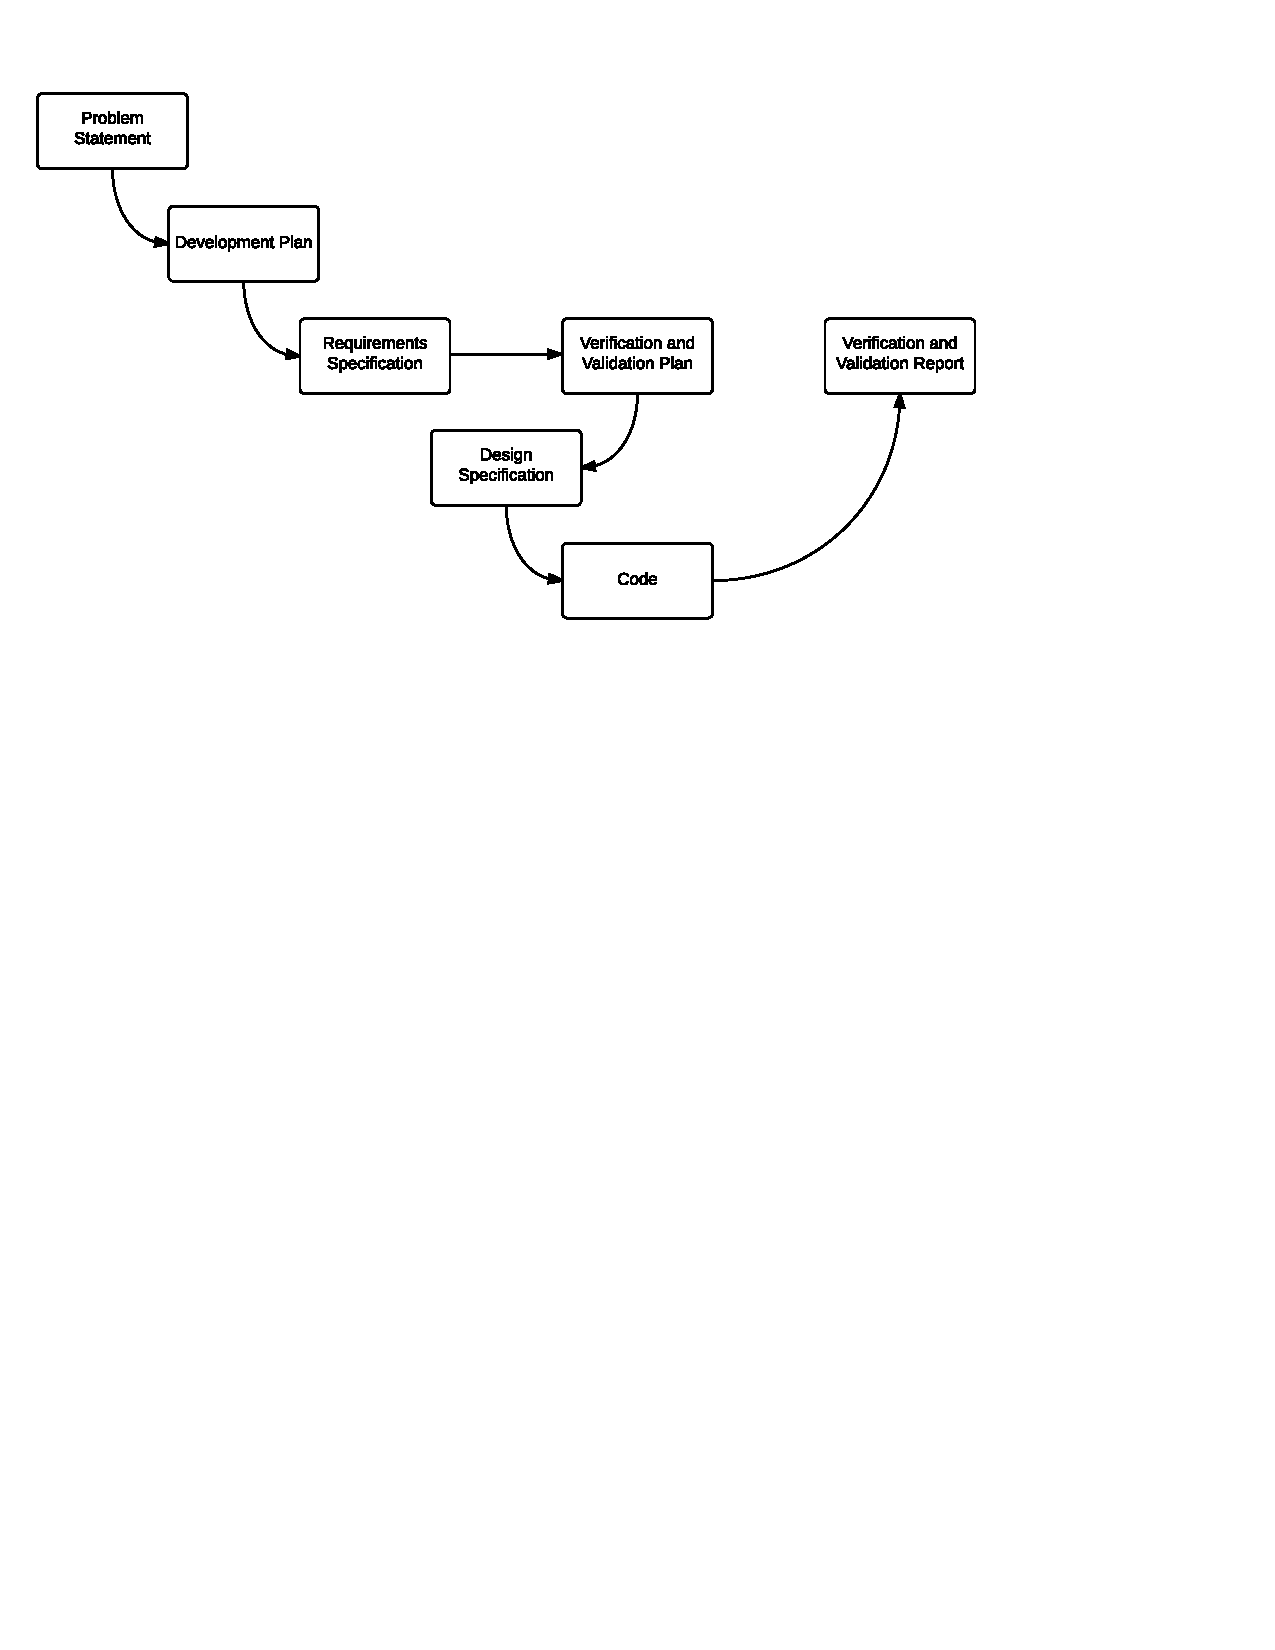
\includegraphics[scale=0.55]{OverviewOfProcess.pdf}
\end{center}

\end{frame}

%%%%%%%%%%%%%%%%%%%%%%%%%%%%%%%%%%%%%%

\section[DDD Benefits]{DDD Benefits}

%%%%%%%%%%%%%%%%%%%%%%%%%%%%%%%%%%%%%%

\begin{frame}

\frametitle{Benefits of DDD}

\begin{itemize}
\item Improve qualities
\begin{itemize}
\item Verifiability
%\item Usability
\item Maintainability
\item Reusability
%\item Understandability
\item Reproducibility
\end{itemize}
\item Better communication
% \item More useful design reviews
% \item More effective code inspections
% \item More effective testing
\item How and Why to Fake It (Parnas and Clements, 1996)
\end{itemize}
\end{frame}

%%%%%%%%%%%%%%%%%%%%%%%%%%%%%%%%%%%%%%

\section[Challenges]{Challenges for DDD}

%%%%%%%%%%%%%%%%%%%%%%%%%%%%%%%%%%%%%%

\begin{frame}

\frametitle{Reasons  ``Manual'' DDD is Unpopular}

\begin{itemize}
\item Up front requirements are challenging
\item Rapid change for numerical algorithms
\item Information duplication
\item Synchronization headaches between artifacts
\item Perceived over-emphasis on non-executable artifacts
%Parnas paper - people do not like docs, vicious cycle
\end{itemize}
\end{frame}

%%%%%%%%%%%%%%%%%%%%%%%%%%%%%%%%%%%%%%

\section[Solution]{Solution -- Knowledge Based Approach (KBA)}

%%%%%%%%%%%%%%%%%%%%%%%%%%%%%%%%%%%%%%

\begin{frame}

\frametitle{Knowledge Based Approach}

\begin{itemize}
\item Capture knowledge
\item From one ``source'' recipes to generate artifacts
\item Automated
\item Inspired by Knuth's Literate Programming
\end{itemize}
\end{frame}

%%%%%%%%%%%%%%%%%%%%%%%%%%%%%%%%%%%%%%

\subsection[Addresses Challenges]{Addresses Challenges}

%%%%%%%%%%%%%%%%%%%%%%%%%%%%%%%%%%%%%%

\begin{frame}

\frametitle{How Addresses Challenges}

\begin{itemize}
\item Supports changing requirements and design
\begin{itemize}
\item Generation
\item Automated traceability
\end{itemize}
\item Supports duplication 
\begin{itemize}
\item Knowledge is entered once, generated/transformed% as required
\item Eases maintenance
\item If incorrect, incorrect everywhere
\end{itemize}
\item Non-executable artifacts are generated
\end{itemize}
\end{frame}

%%%%%%%%%%%%%%%%%%%%%%%%%%%%%%%%%%%%%%

\subsection[Benefits]{Benefits}

%%%%%%%%%%%%%%%%%%%%%%%%%%%%%%%%%%%%%%

\begin{frame}

\frametitle{Verifiability}

\begin{table} 
\centering
%\caption{Constraints on quantities}
\begin{tabular}{c c r c } 
\toprule
\textbf{Var} & \textbf{Constraints} & \textbf{Typical Value} & \textbf{Uncertainty}\\ \midrule
$L$ & $L > 0$ & 1.5 m & 10\% \\ 
$D$ & $D > 0$ & 0.412 m & 10\% \\ 
$V_P$ & $V_P > 0$ & 0.05 m$^3$	& 10\% \\
$A_P$ & $A_P > 0$ & 1.2 m$^2$	& 10\% \\
$\rho_P$ & $\rho_P > 0$	& 1007 kg/m$^3$	& 10\% \\
\bottomrule
\end{tabular}
\label{tab:pcm}
\end{table}

\begin{itemize}
\item Sanity checks captured and reused
\item Generate guards against invalid input
\item Generate test cases
\end{itemize}
\end{frame}

%%%%%%%%%%%%%%%%%%%%%%%%%%%%%%%%%%%%%%

\begin{frame}

\frametitle{Reusability}

 \noindent
\begin{minipage}{\columnwidth}
\begin{tabular}{@{} p{\colAwidth}  p{\colBwidth}@{}}
\toprule
\textbf{Number}& \textbf{T1} \\
\midrule
Label&\bf Conservation of energy\\
\midrule
Equation&  $-{\bf \nabla \cdot q} +q'''$ = $\rho C \frac{\partial T}{\partial t}$ \smallskip\\
\midrule
Description & The above equation gives the conservation of energy for time 
varying heat transfer in a material of specific heat capacity $C$ and density $\rho$,
where $\bf q$ is the thermal flux vector, $q'''$ is the volumetric heat
generation, $T$ is the temperature, $\nabla$ is the del operator and $t$ is the time.\\
\bottomrule
\end{tabular}
\end{minipage}

\end{frame}

%%%%%%%%%%%%%%%%%%%%%%%%%%%%%%%%%%%%%%

\begin{frame}

\frametitle{Usability}

\begin{itemize}
\item As simple as possible, but not simpler (Einstein)
\item Usability challenges for general purpose SCS
\begin{itemize}
\item Complex, confusing
\item Generic symbols and terminology
\end{itemize}
\item Generate apps suited to specific scientific and engineering needs
\item Finite element software example
\end{itemize}
\end{frame}

%%%%%%%%%%%%%%%%%%%%%%%%%%%%%%%%%%%%%%

\begin{frame}

\frametitle{Reproducibility}

\begin{itemize}
\item Knowledge is explicitly stored for the future
\item Recipes can be use to regenerate any artifacts
\item Recipes include build instructions
\end{itemize}
\end{frame}

%%%%%%%%%%%%%%%%%%%%%%%%%%%%%%%%%%%%%%

\begin{frame}

\frametitle{Software Certification}

\begin{itemize}
\item Recertification can be expensive and time consuming
\item Change propagates through documentation
\item Traceability and maintainability
\item Recipes help with changing documentation standards
\end{itemize}

\end{frame}

%%%%%%%%%%%%%%%%%%%%%%%%%%%%%%%%%%%%%%

\section[Feasibility]{Feasibility (Introducing Drasil)}

%%%%%%%%%%%%%%%%%%%%%%%%%%%%%%%%%%%%%%

\begin{frame}

\frametitle{Drasil Framework Design}

\begin{center}
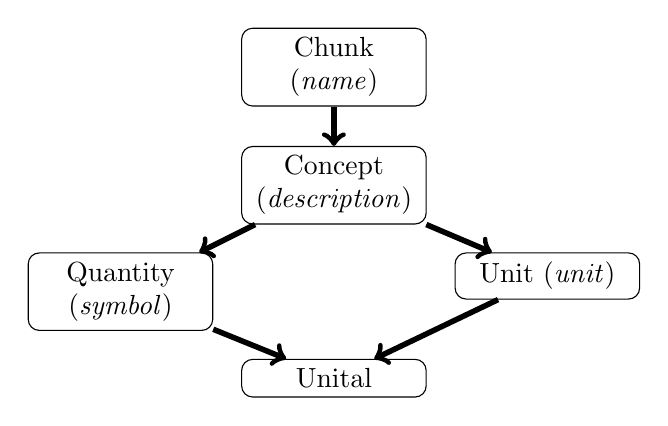
\begin{tikzpicture}[node distance=5mm]
  \tikzstyle{every node}=[draw,shape=rectangle, rounded corners,
    text width=6em, text centered];
  \node (ch)                     {Chunk (\emph{name})};
  \node (co) [below = of ch]       {Concept (\emph{description})};
  \node (qu) [below left = of co]  {Quantity (\emph{symbol})};
  \node (u ) [below right = of co] {Unit (\emph{unit})};
  \node (uc) [below right = of qu] {Unital};

  \draw [->, line width=2pt] (ch) -- (co);
  \draw [->, line width=2pt] (co) -- (qu);
  \draw [->, line width=2pt] (co) -- (u );
  \draw [->, line width=2pt] (qu) -- (uc);
  \draw [->, line width=2pt] (u ) -- (uc);
\end{tikzpicture}
\end{center}

\end{frame}

%%%%%%%%%%%%%%%%%%%%%%%%%%%%%%%%%%%%%%

\begin{frame}[fragile]

%\frametitle{Excerpt from SRS}

\begin{center}
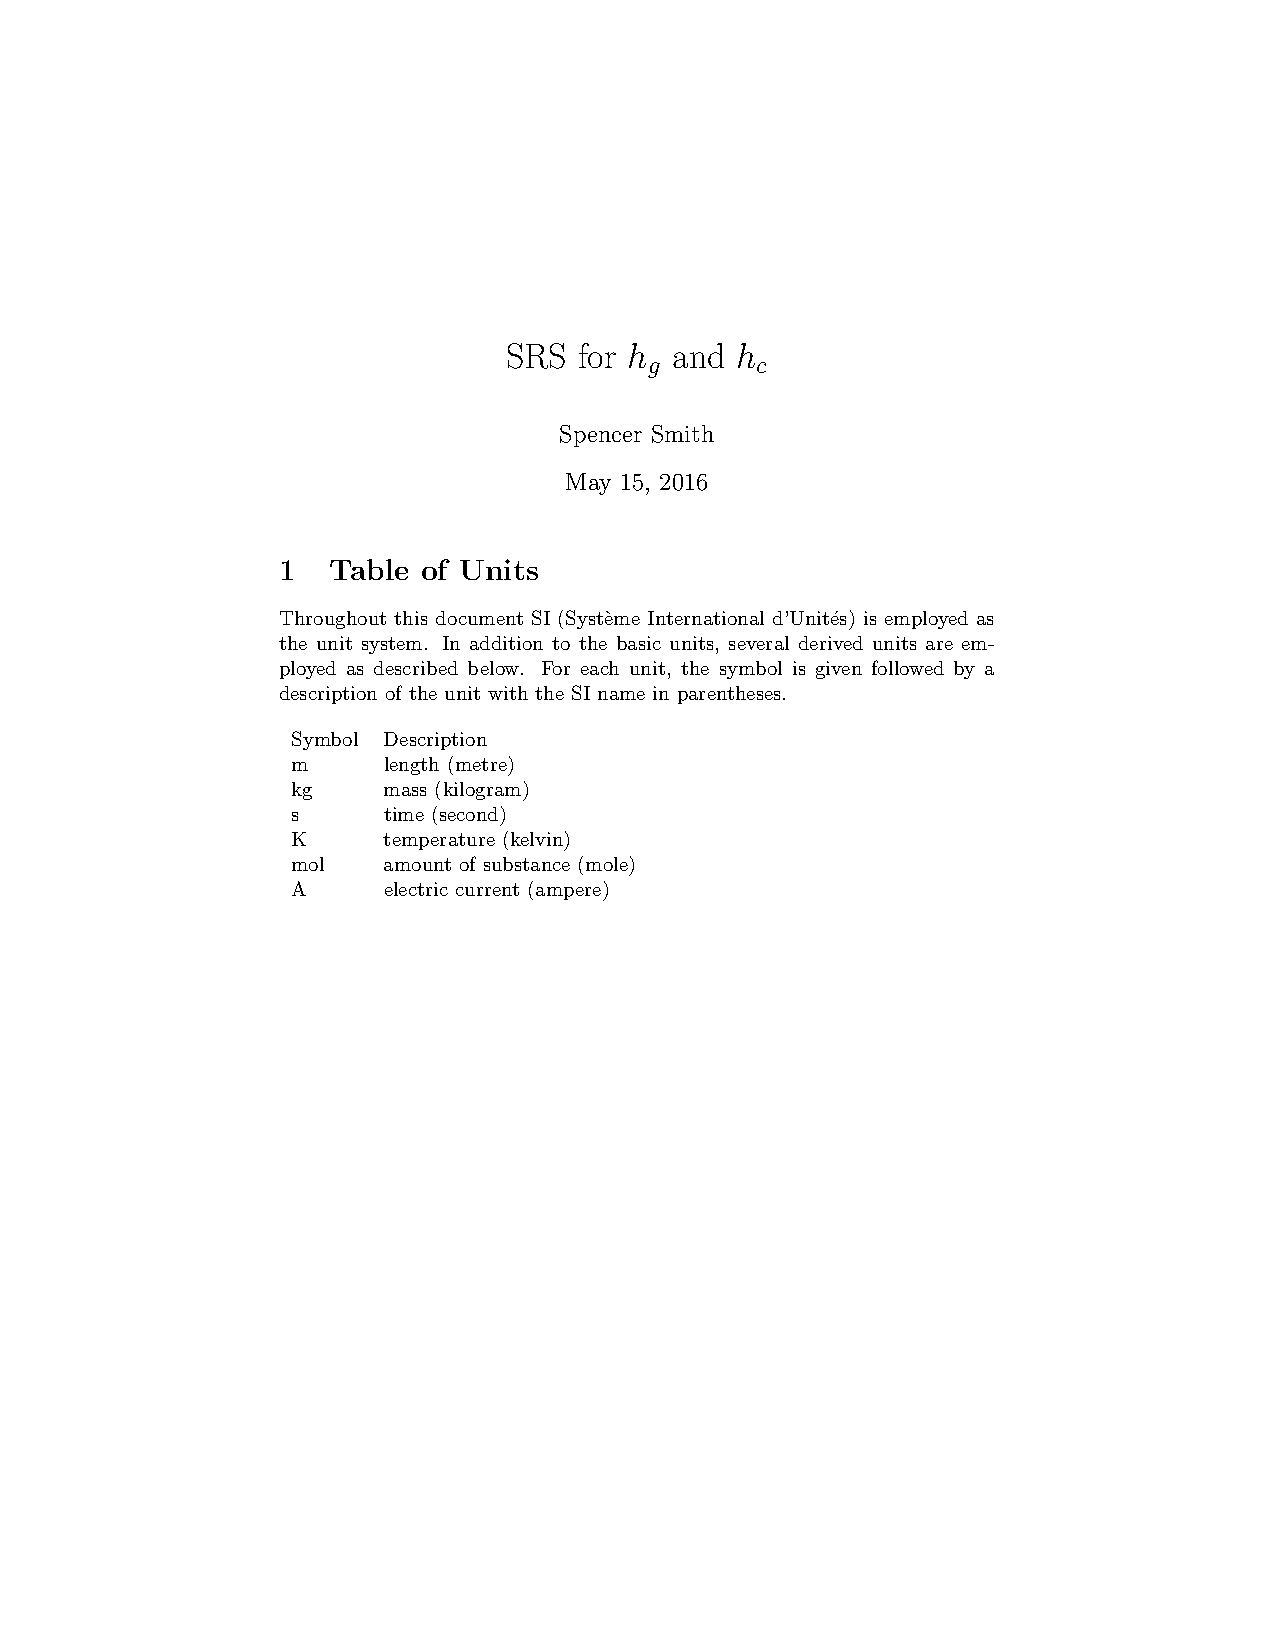
\includegraphics[scale=0.8]{SRS_Excerpt.pdf}
\end{center}
\end{frame}

%%%%%%%%%%%%%%%%%%%%%%%%%%%%%%%%%%%%%%
\begin{frame}[fragile]

\frametitle{Example Recipe}

\begin{lstlisting}[frame=none, 
  showstringspaces=false, basicstyle=\small]
srsBody = srs [h_g, h_c] "Spencer Smith" [s1,s2]

s1 = Section (S "Table of Units") [intro, table]

table = Table 
 [S "Symbol", S "Description"] (mkTable
   [(\x -> Sy (x ^. unit)),
    (\x -> S (x ^. descr)) ] si_units)

intro = Paragraph (S "Throughout this ...")
\end{lstlisting}
\end{frame}

%%%%%%%%%%%%%%%%%%%%%%%%%%%%%%%%%%%%%%

\begin{frame}[fragile]

\frametitle{Reusable Chunks}

\begin{lstlisting}[frame=none, showstringspaces=false, 
  basicstyle=\small]
metre, second, kelvin :: FundUnit
metre  = fund "Metre"  "length (metre)"       "m"
second = fund "Second" "time (second)"        "s"
kelvin = fund "Kelvin" "temperature (kelvin)" "K"
\end{lstlisting}

\end{frame}

%%%%%%%%%%%%%%%%%%%%%%%%%%%%%%%%%%%%%%

\begin{frame}[fragile]

\frametitle{The $h_c$ Chunk}

$$h_{c} = \frac{2k_{c} h_{b}}{2k_{c}+\tau_{c}h_{b}}$$
~\newline

\begin{lstlisting}[frame=none, showstringspaces=false, basicstyle=\small]
h_c_eq :: Expr
h_c_eq = 2*(C k_c)*(C h_b) /
  (2*(C k_c) + (C tau_c)*(C h_b))

h_c :: EqChunk
h_c = fromEqn "h_c" 
 "convective heat transfer coefficient between 
    clad and coolant"
   (sub h c) heat_transfer h_c_eq

\end{lstlisting}

\end{frame}

%%%%%%%%%%%%%%%%%%%%%%%%%%%%%%%%%%%%%%

\section[Future Work]{Future Work}

%%%%%%%%%%%%%%%%%%%%%%%%%%%%%%%%%%%%%%

\begin{frame}

\frametitle{Next Steps}

\begin{itemize}
\item Generate more artifact types
\item Generate different document views
\item More types of information in chunks
\item Use constraints to generate test cases
\item Implement larger examples
\end{itemize}

\end{frame}

%%%%%%%%%%%%%%%%%%%%%%%%%%%%%%%%%%%%%%

\section[Conclusions]{Conclusions}

%%%%%%%%%%%%%%%%%%%%%%%%%%%%%%%%%%%%%%

\begin{frame}

\frametitle{Conclusions}

\begin{itemize}
\item SCS has the opportunity to lead other software fields by leveraging its
  solid existing knowledge base
\item DDD is feasible with a knowledge-based approach
\item Documentation for QA and software certification does not have to be
  painful, expensive or time consuming
\item Drasil will be developed via practical case studies
\end{itemize}
\end{frame}

%%%%%%%%%%%%%%%%%%%%%%%%%%%%%%%%%%%%%%

\end{document}